\documentclass[9pt,a4paper]{tau-class/tau}
\usepackage{dirtree}
\usepackage{graphicx} % Required for inserting images
\usepackage[utf8]{inputenc}
\usepackage[brazilian]{babel}
\usepackage{amsmath}
\usepackage{minted}
\usepackage{pgfplots}
\usepackage{algpseudocode}
\usepackage{float}
\usepackage{fancyhdr}
\usepackage{algorithm}
\usepackage{tikz-cd} 
\usepackage{amsthm}
\usepackage{tikz}
\usepackage{hyperref}
\usepackage{amsfonts}
\usepackage{url}
%\usepackage{amssymb}
\usepackage{mathrsfs}
\usepackage[thinc]{esdiff}
\usepackage{ragged2e}
\usepackage{graphicx}
\usepgfplotslibrary{external}
\pgfplotsset{compat=1.18}
\setcounter{tocdepth}{4}
\setcounter{secnumdepth}{4}
\DeclareMathOperator\sen{sen}
\theoremstyle{definition}
%% Spanish babel recomendation
% \usepackage[spanish,es-nodecimaldot,es-noindentfirst]{babel} 

%% Draft watermark
% \usepackage{draftwatermark}

%----------------------------------------------------------
% TITLE
%----------------------------------------------------------

\journalname{Arthur H. Sandonato - arthur.sandonato@usp.br - 15441240}
\title{Introdução ao Caos - AA1}

%----------------------------------------------------------
% AUTHORS, AFFILIATIONS AND PROFESSOR
%----------------------------------------------------------

\author{}

%----------------------------------------------------------
% FOOTER INFORMATION
%----------------------------------------------------------

\footinfo{}
\theday{{}}

%----------------------------------------------------------
\bibliography{tau}
\newtheorem{definition}{Definição}
\newtheorem{theorem}{Teorema}
\newtheorem{observation}{Observação}
\newtheorem{example}{Exemplo}
\newtheorem{lemma}{Lema}
\renewcommand{\proofname}{Demonstração}
\numberwithin{definition}{subsection}
\numberwithin{theorem}{subsection}
\numberwithin{example}{subsection}
\numberwithin{observation}{subsection}
\numberwithin{lemma}{subsection}
\renewcommand{\thesubsection}{\thesection\alph{subsection})}
\renewcommand{\thesubsubsection}{\thesubsection\roman{subsubsection})}

\begin{document}	
    \maketitle 
    \thispagestyle{firststyle} 
    %\linenumbers 
    \pagestyle{fancy}
\fancyhf{} % Limpa os cabeçalhos padrão
\rfoot{
\includegraphics[height=1cm]{logo.png}} % Logo no topo direito
\renewcommand{\headrulewidth}{0pt} % Remove a linha do cabeçalho (opcional)
\tableofcontents

\section{Pontos fixos e retratos de fase}

\subsection{Sistema linear I}

Selecionando o sistema linear

    \[\begin{cases}
        \dot{x} = -3x \\ 
        \dot{y} = 3x - 2y
    \end{cases}\]

    Podemos escrever $\vec{\dot{x}} = M\vec{x}$, onde

    \[\vec{x} = \begin{bmatrix} 
    x \\ 
    y
    \end{bmatrix}; \vec{\dot{x}} = \begin{bmatrix}
        \dot{x} \\
        \dot{y}
    \end{bmatrix}; M = \begin{bmatrix}
        -3 & 0 \\
        3 & -2
    \end{bmatrix}\]

    Os pontos fixos satisfazem $\vec{\dot{x}} = 0$. Como $M \neq 0$, os pontos fixos são $x^* = y^* = 0$.

    Pra avaliar a estabilidade dos pontos fixos, podemos calcular os autovalores de $M$ através das raízes do polinômio característico 

    \[\det(M - \lambda I) = 0 \iff \begin{vmatrix}
        -3 - \lambda & 0 \\
        3 & -2 - \lambda
    \end{vmatrix} = 0 \Rightarrow (\lambda + 2)(\lambda + 3) = 0 \iff \begin{cases}
        \lambda = -2 \\ 
        \lambda = -3
    \end{cases}\]

    Como ambos os autovalores são reais e negativos, o ponto fixo identificado é estável. Podemos determinar os autovetores associados a cada autovalor, também 

    \begin{itemize}
        \item $\lambda = -2$: 

        \[(A + 2I)\vec{v}_{-2} = 0 \iff \begin{bmatrix}
            -1 & 0 \\
            3 & 0 
        \end{bmatrix}\begin{bmatrix}
            a \\
            b
        \end{bmatrix} = 0 \iff a = 0, b \in \mathbb{R}_*\]

        Podemos selecionar, por conveniência, 

        \[\vec{v}_{-2} = \begin{bmatrix}
            0 \\
            1
        \end{bmatrix}\]

        \item $\lambda = -3$: 

        Similarmente, def. $\vec v_{-3} = \begin{bmatrix}
            u & v
        \end{bmatrix}^T$, temos $(A + 3I)\vec v_{-3} = 0 \iff $
        \[\iff \begin{bmatrix}
            0 & 0 \\
            3 & 1
        \end{bmatrix}\begin{bmatrix}
            u \\
            v
        \end{bmatrix} = 0 \iff v = -3u\]

        Para $u = 1$, $v = -3$, e uma escolha possível é 

        \[\vec v_{-3} = \begin{bmatrix}
            1 \\
            -3 
        \end{bmatrix}\]
        
    \end{itemize}

    Por meio das equações do sistema, podemos gerar soluções gerais para as EDOs. Para $x$, $x(t) = x_0 e^{-3t}$, então $\dot{y} + 2y = 3x_0e^{-3t}$. Tomando $y = y_h + y_p$, podemos resolver a EDO homogênea 

    \[\dot{y}_h + 2y_h = 0 \iff y_h = y_0 e^{-2t}\]

    Para a solução particular, considere $y_p = K e^{-3t}$, e 

    \[\dot{y}_p + 2y_p = 3x_0 e^{-3t} = -3Ke^{-3t} + 2Ke^{-3t} = -3x_0e^{-3t} \overset{t \to \infty}{\longrightarrow} -3K + 2K = -3x_0 \iff K = -3x_0\]

    Ou seja, 

    \[y(t) = (y_0 + 3x_0)e^{-2t} - 3x_0e^{-3t} = x_0e^{-3t}\cdot\vec{v}_{-3} + (y_0 + 3x_0)e^{-2t}\cdot\vec{v}_{-2}\]

    Com isso, podemos esboçar o retrato de fase desse sistema, como na fig. \ref{fig:1a}.

    \begin{figure}[H]
        \centering
        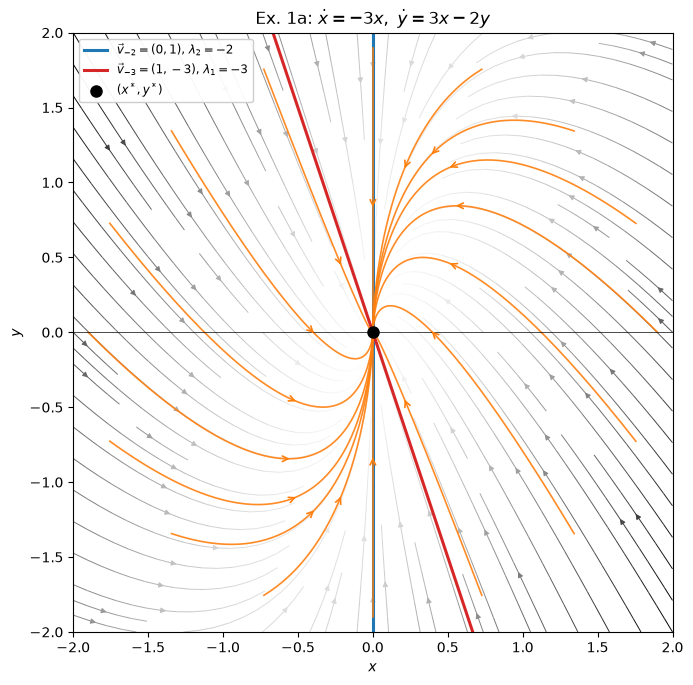
\includegraphics[width=0.5\linewidth]{1a.png}
        \caption{Retrato de fase do sistema $\dot{x} = -3x$, $\dot{y} = 3x - 2y$.}
        \label{fig:1a}
    \end{figure}

\subsection{Sistema linear II}

Escolhendo 

\[\begin{cases}
    \dot{x} = -x + y \\ 
    \dot{y} = -4x + y
\end{cases}\]

    Podemos realizar o mesmo tratamento que previamente. Primeiro, tomando 

    \[\vec x= \begin{bmatrix}
        x \\ 
        y
    \end{bmatrix}, \vec{\dot{x}} = \begin{bmatrix}
        \dot{x} \\ 
        \dot{y}
    \end{bmatrix}, M = \begin{bmatrix}
        -1 & 1 \\ 
        -4 & 1
    \end{bmatrix}\]

    Para termos $\vec{\dot{x}} = 0$, devemos ter $x = y$, e $4x = y \iff x= y = 0 $. 

    Os autovalores associados a $M$ serão as raízes do polinômio característico 

    \[\begin{vmatrix}
        -1 - \lambda & 1 \\ 
        -4 & 1 - \lambda
    \end{vmatrix} = 0 \iff \lambda^2 + 3  = 0 \iff \lambda_{\pm} = \pm i\sqrt{3}\]

    Como a parte real dos autovalores é zero, eles apresentam rotação, mas com curvas fechadas, no espaço de fases. Se avaliarmos o sistema nos pontos $(1,0)$, $(0,1)$, teremos 

    \[\begin{cases}
        \dot{x}(1,0) = -1 \\ 
        \dot{y}(1,0) = -4 \\ 
        \dot{x}(0,1) = 1 \\ 
        \dot{y}(0,1) = 1 
    \end{cases}\]

Ou seja, estamos indo $\begin{bmatrix}
    -1 & -4
\end{bmatrix} \to \begin{bmatrix}
    1 & 1
\end{bmatrix}$, ou seja, a rotação é no sentido horário. 

Podemos determinar a solução explícita considerando as EDOs fornecidas. Para $\dot{x}$, podemos fazer 

\[\ddot{x} = -\dot{x} + \dot{y} = -\dot{x} - 4x + y\]

    Mas, $y = \dot{x} + x$, então 

    \[\ddot{x} = -3x \iff x(t) = x_0\cos\omega t + \frac{y_0 - x_0}{\omega}\cdot\sen\omega t\]

    considerando o estado inicial como $(x_0, y_0)$. A partir disso, $y(t) = \dot{x} + x$.

    Com isso, podemos esboçar o retrato de fase do sistema, como na fig. \ref{fig:1b}.

    \begin{figure}[H]
        \centering
        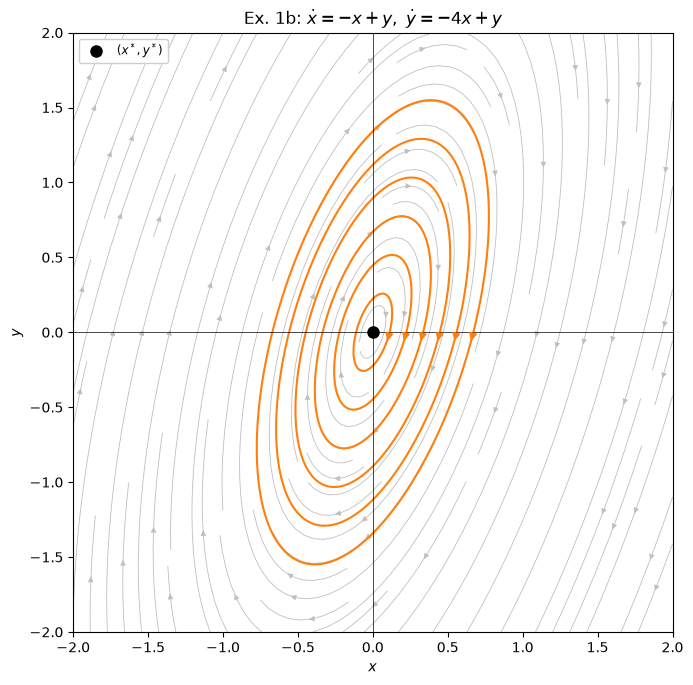
\includegraphics[width=0.5\linewidth]{1b.png}
        \caption{Retrato de fase do sistema escolhido.}
        \label{fig:1b}
    \end{figure}

\subsection{Sistema não linear}

Os pontos fixos ocorrerão quando $(\dot{x}, \dot{y}) = 0 \iff $

    \[\begin{cases}
        x = 0, \text{ ou } x + 2y = 3 \\
        y = 0, \text{ ou } x + y = 2
    \end{cases}\begin{cases}
        x = y = 0 \Rightarrow (x^*, y^*) = (0,0) \\ 
        x = 0, x + y = 2 \Rightarrow (x^*, y^*) = (0,2) \\ 
        y = 0, x + 2y = 3 \Rightarrow (x^*, y^*) = (3,0) \\ 
        x + 2y = 3, x + y = 2 \Rightarrow \begin{cases}
            x^* + 2y^* = 3 \\
            x^* + y^* = 2
        \end{cases} \iff (x^*, y^*) = (1,1)
    \end{cases}\]

    Denominando $f(x,y) = \dot{x}$, $g(x,y) = \dot{y}$, podemos escrever a jacobiana

    \[J(x,y) = \begin{bmatrix}
        \partial_xf & \partial_y f \\ 
        \partial_xg & \partial_yg
    \end{bmatrix} = \begin{bmatrix}
        3 - 2x - 3y & -2x \\
        -y & 2 - x - 2y
    \end{bmatrix}\]

    Avaliando em cada ponto, teremos 

    \begin{itemize}
        \item $(0,0)$: 

        \[J = \begin{bmatrix}
        3 & 0 \\ 
        0 & 2
        \end{bmatrix} \Rightarrow \begin{cases}
            \lambda = 3 \\ 
            \lambda = 2
        \end{cases}\]

        Como ambos são positivos e reais, o ponto fixo é instável. 

        \item $(0,2)$:

        \[J = \begin{bmatrix}
            -1 & 0 \\ 
            -2 & -2
        \end{bmatrix}\]

        Disso, podemos avaliar o polinômio característico associado a essa jacobiana 

        \[\begin{vmatrix}
            -1 - \lambda & 0 \\
            -2 & -2 - \lambda
        \end{vmatrix} = 0 \iff \begin{cases}
            \lambda = -1 \\
            \lambda = -2
        \end{cases}\]

        Como ambos são negativos e reais, o ponto fixo é estável. 

        \item $(3,0)$: 

        \[J = \begin{bmatrix}
            -3 & -6 \\
            0 & -1
        \end{bmatrix}\]

        Disso, 

        \[\begin{vmatrix}
            -3 -\lambda & -6 \\
            0 & -1 - \lambda
        \end{vmatrix} = 0 \iff \begin{cases}
            \lambda = -3 \\ 
            \lambda = - 1
        \end{cases}\]

        Como ambos são reais e negativos, o ponto fixo é estável. 

        \item $(1,1)$:

        \[J = \begin{bmatrix}
            -1 & -2 \\
            -1 & -1 
        \end{bmatrix}\]

        Disso, 

        \[\begin{vmatrix}
            -1 - \lambda & -2 \\ 
            -1 & -1 - \lambda
        \end{vmatrix} = 0 \iff (1 + \lambda)^2 = 2 \iff \lambda_\pm = -1 \pm \sqrt{2}\]

        Nesse caso, como temos um autovalor positivo e um negativo, e ambos reais, temos um ponto de sela. 
        
    \end{itemize}

    Podemos esboçar o espaço de fase a partir das EDOs, sem uma solução geral, tal qual a fig. \ref{fig:1c}

    \begin{figure}[H]
        \centering
        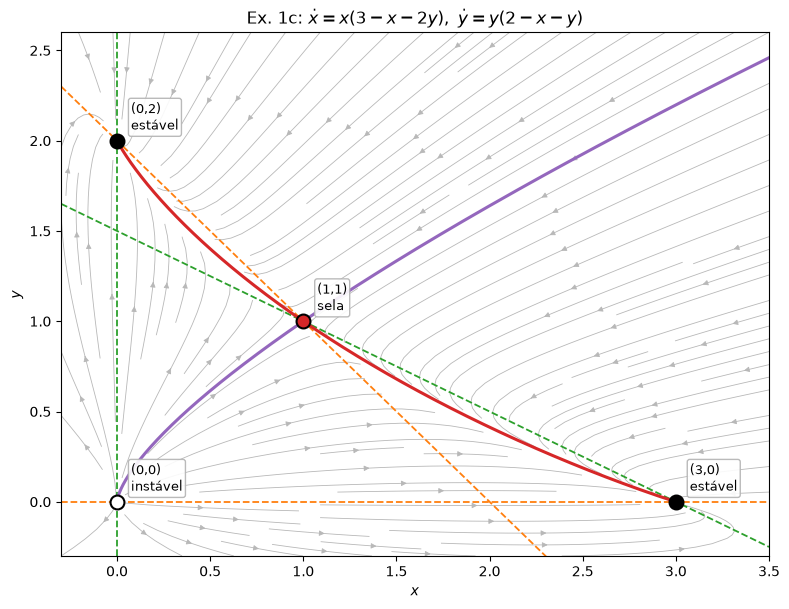
\includegraphics[width=0.5\linewidth]{1c.png}
        \caption{Retrato de fase do sistema em questão.}
        \label{fig:1c}
    \end{figure}

    \begin{figure}[H]
        \centering
        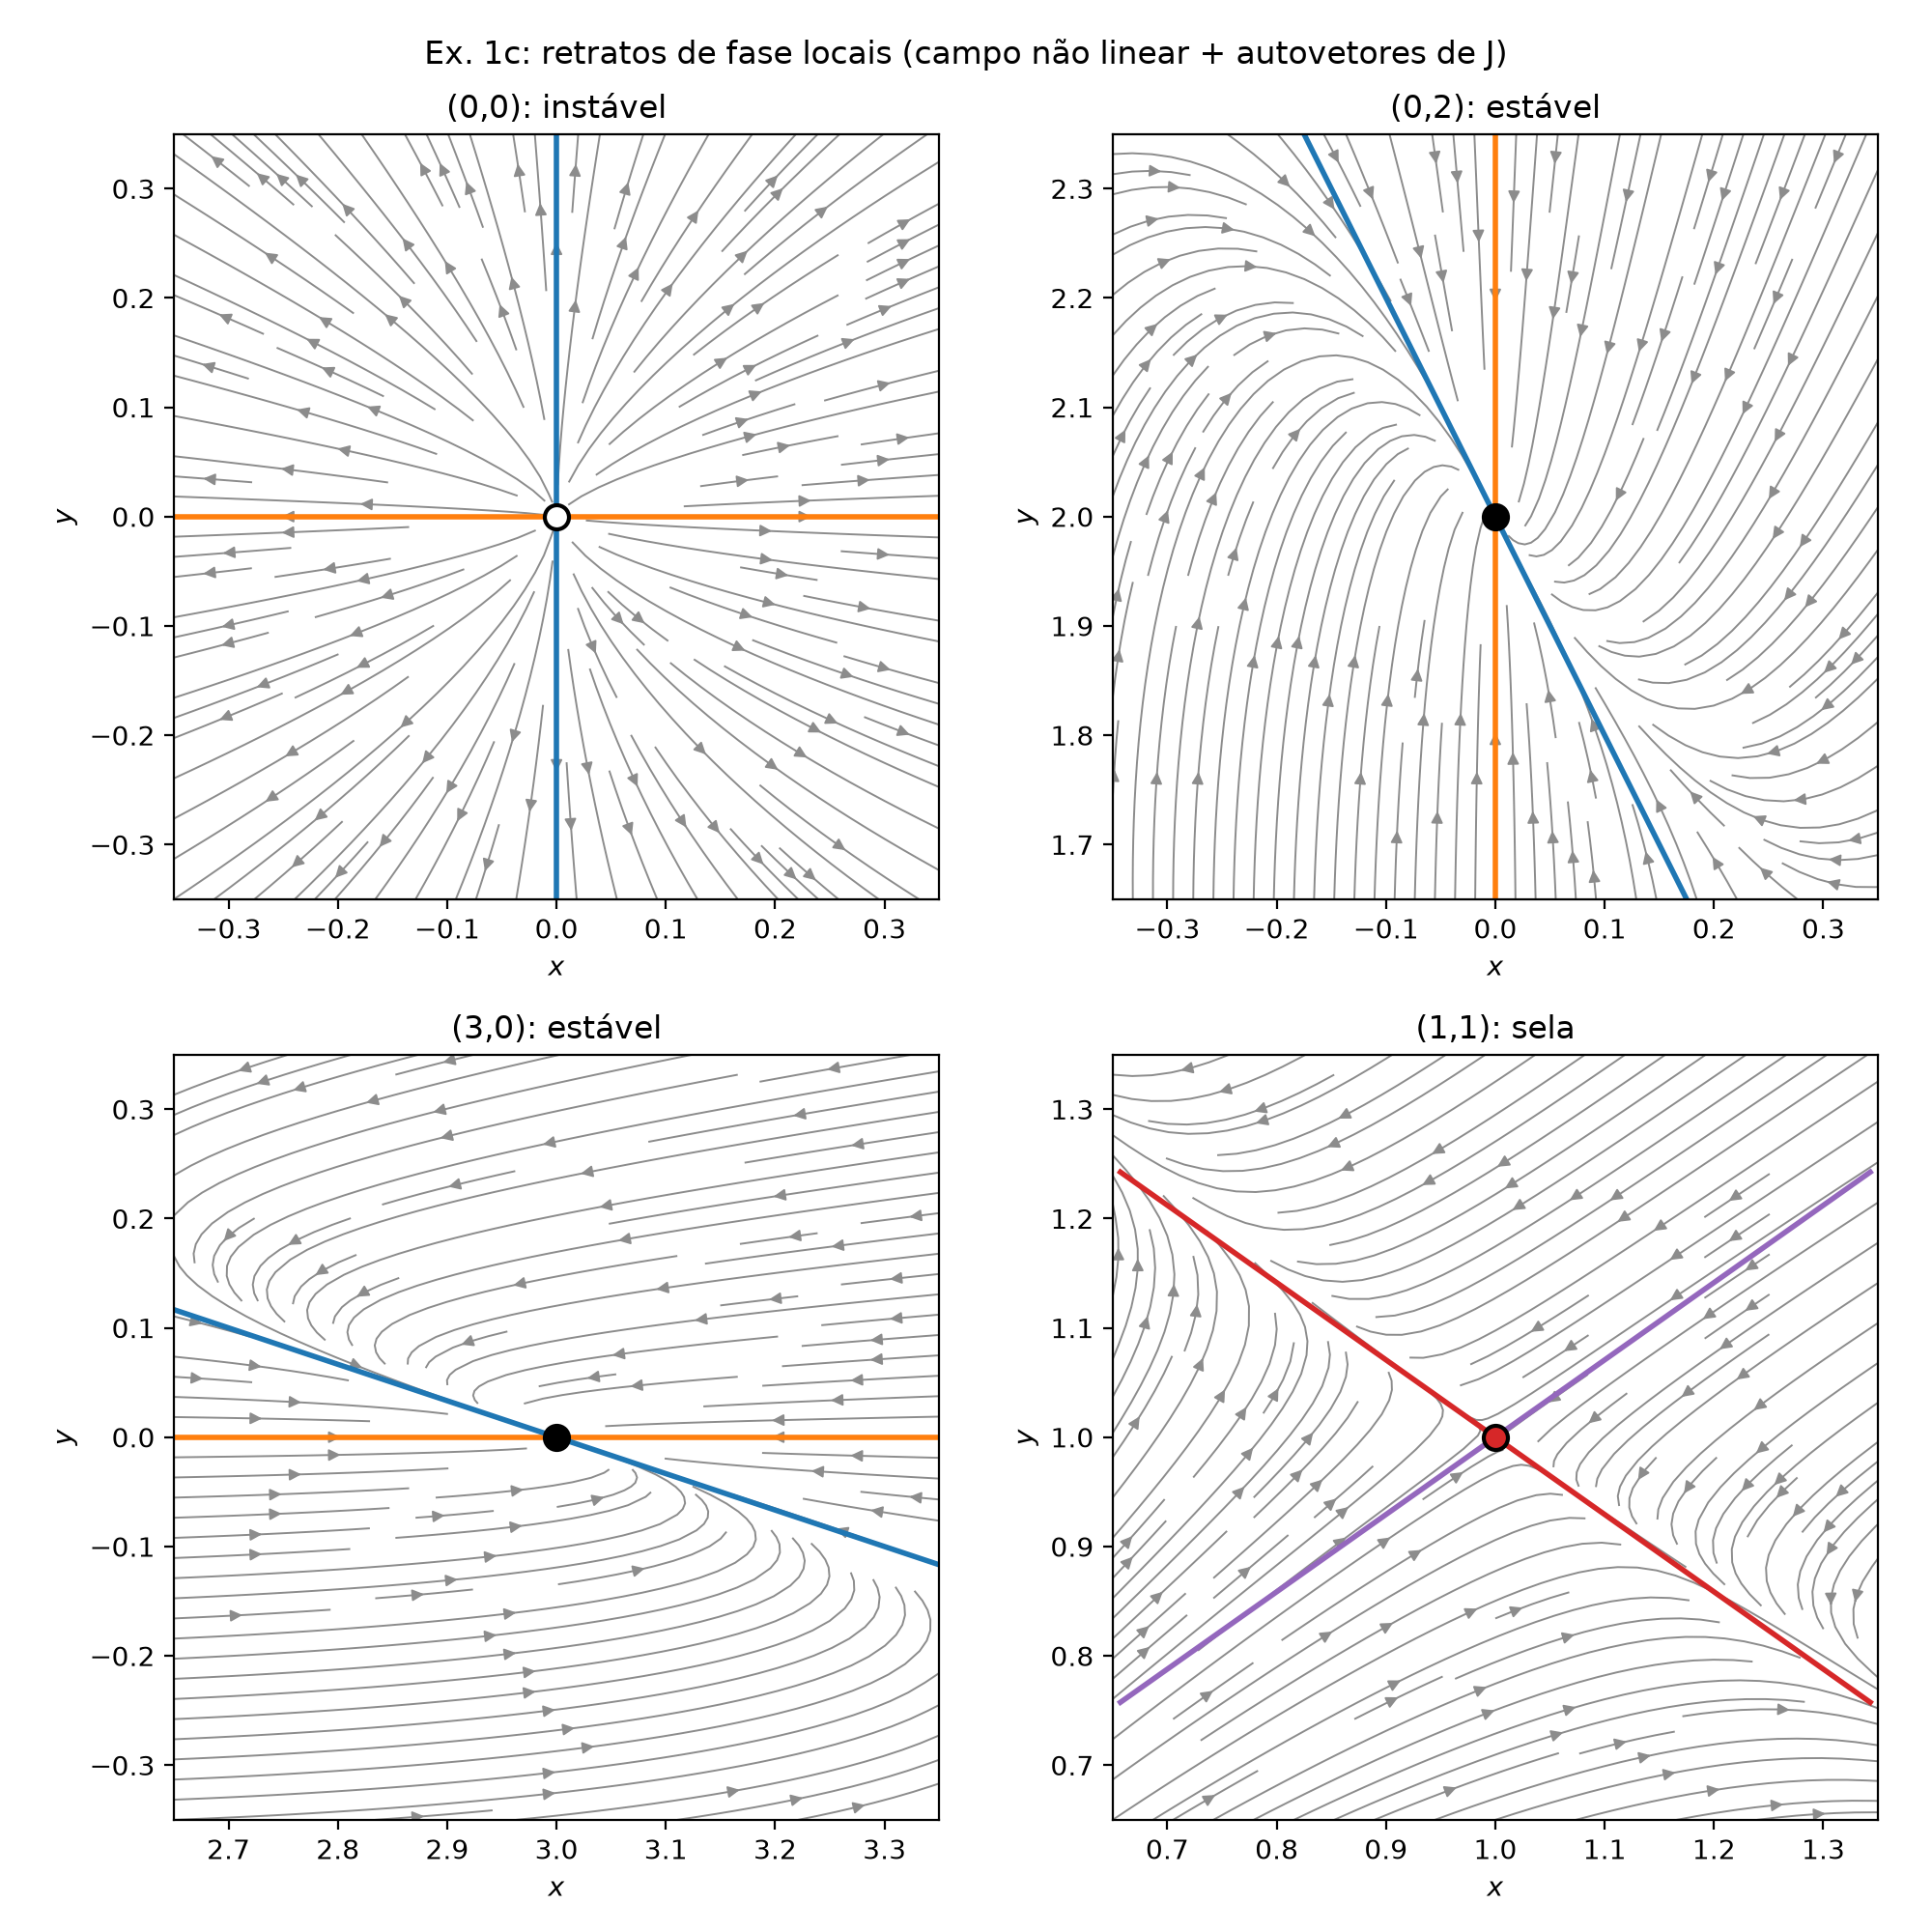
\includegraphics[width=0.5\linewidth]{1c_loc.png}
        \caption{Retratos de fase locais, para cada ponto fixo identificado.}
        \label{fig:1c_loc}
    \end{figure}

\section{Pêndulo e aproximação para amplitudes moderadas}

Definindo $f(\theta) = -\theta + \frac{\theta^3}{6}$, os pontos fixos serão em $f(\theta^*) = 0$, para algum $\theta^*$. Para isso, devemos ter 

\[\theta^*(-1 + (\theta^*)^2/6) = 0 \iff \begin{cases}
    \theta^* = 0 \\ 
    \theta^* = \pm \sqrt{6}
\end{cases}\]

A jacobiana é, então, 

\[J = \begin{bmatrix}
    0 & 1 \\ 
    f'(\theta^*) & 0 
\end{bmatrix}, \text{ onde }f'(\theta) = -1 + \frac{\theta^2}{2}\]
    
    Assim, as raízes do polinômio característico são 

    \[\begin{vmatrix}
        - \lambda & 1 \\ 
        f'(\theta^*) & -\lambda
    \end{vmatrix} = 0 \iff \lambda^2 = f'(\theta^*)\]

    Assim, para 

    \begin{itemize}
        \item $(0,0)$: $f'(\theta^*) = -1$, então $\lambda = \pm i$. Como esses autovalores são imaginários puros, as órbitas são fechadas, e o ponto fixo é um centro. 
        \item $(\pm\sqrt 6, 0)$: $f'(\theta^*) = 2 \iff \lambda = \pm\sqrt{2}$. Como temos um autovalor positivo e um negativo, os pontos fixos são selas. 
    \end{itemize}

    Se considerarmos a equação adimensionalizada original, podemos definir $g(\theta) = -\sen\theta$. Os pontos fixos são em $\sen\theta^* = 0$, ou seja 

    \[\theta^* = 2\pi n, n \in \mathbb{N}\]

    Se permitíssemos $n \in \mathbb{R}$, conseguimos avaliar a proximidade dos pontos fixos. Teríamos, então, que $n = \pm\frac{\sqrt{6}}{2\pi}\cong 0,39$ para que os pontos fixos sejam equivalentes, então, os sistemas são próximos para pequenos ângulos. 

    Ainda nessa mesma linha, podemos escrever a série de Taylor

    \[\sen\theta = \sum_{n=0}^\infty \frac{(-1)^n}{(2n + 1)!}\theta^{2n + 1} = -\theta + \frac{1}{6}\theta^3 + \mathcal{O}(\theta^5)\]

    De tal modo que, para pequenos ângulos tenhamos, de fato 

    \[\sen\theta \cong \theta - \frac{\theta^3}{6} \Rightarrow \ddot{\theta}= -\sen\theta \cong -\theta + \frac{1}{6}\theta^3\]

    Podemos analisar esse mesmo sistema sob a perspectiva da energia se definirmos as energias potenciais 

    \[V'_f(\theta) = -f(\theta) \iff V_f(\theta) = \frac{\theta^2}{2} - \frac{\theta^4}{24}\]
    \[V_g(\theta) = 1 - \cos\theta \]

    assumindo $V(0) = 0$ para ambos os casos. Desse modo, 

\[\ddot{\theta} = -V'(\theta) \Rightarrow \ddot{\theta}\theta + \theta V' = 0 \Rightarrow \frac{d}{dt}\left [ \frac{\dot{\theta}^2}{2} + V(\theta)\right ] = 0 \]

Assim, como o sistema é conservativo, podemos definir $E := \frac{\dot{\theta}^2}{2}+ V(\theta) = $ cte. Disso, no ponto de retorno, $E = V(A)$, onde $A$ é a amplitude de oscilação, e disso 

\[\dot{\theta} = \pm \sqrt{2(V(A) - V(\theta))} \Rightarrow T(A) = 4 \int_0^A\frac{d\theta}{\sqrt{2[V(A) - V(\theta)]}}\]

Para $g$, é \href{https://ed.quantum-bg.org/elliptic-integrals.pdf}{conhecido} que $T_g(A) = 4K(k)$, $k = \sen A/2$. Para $f$, podemos escrever 

\[T_f(A) = 4\int_0^{\pi/2}\frac{d\varphi}{\sqrt{1 - \frac{A^2}{12}(1 + \sen^2\varphi)}}\]

De modo que podemos expandir 

\[T_g = 2\pi \left ( 1 + \frac{A^2}{16} + \frac{11A^4}{3072} + \dots \right )\]
\[T_f = 2\pi \left ( 1 + \frac{A^2}{16} + \frac{19A^4}{3072} + \dots \right )\]

A diferença entre os dois métodos, então, se dá, primeiramente, no termo de ordem $\mathcal{O}(A^4)$. Para pequenas amplitudes, portanto, a aproximação, de fato, vale, sob uma perspectiva de período, também. 

Por fim, podemos analisar o retrato de fase, e a diferença visual entre os dois períodos, na fig. \ref{fig:2}.

\begin{figure}[H]
    \centering
    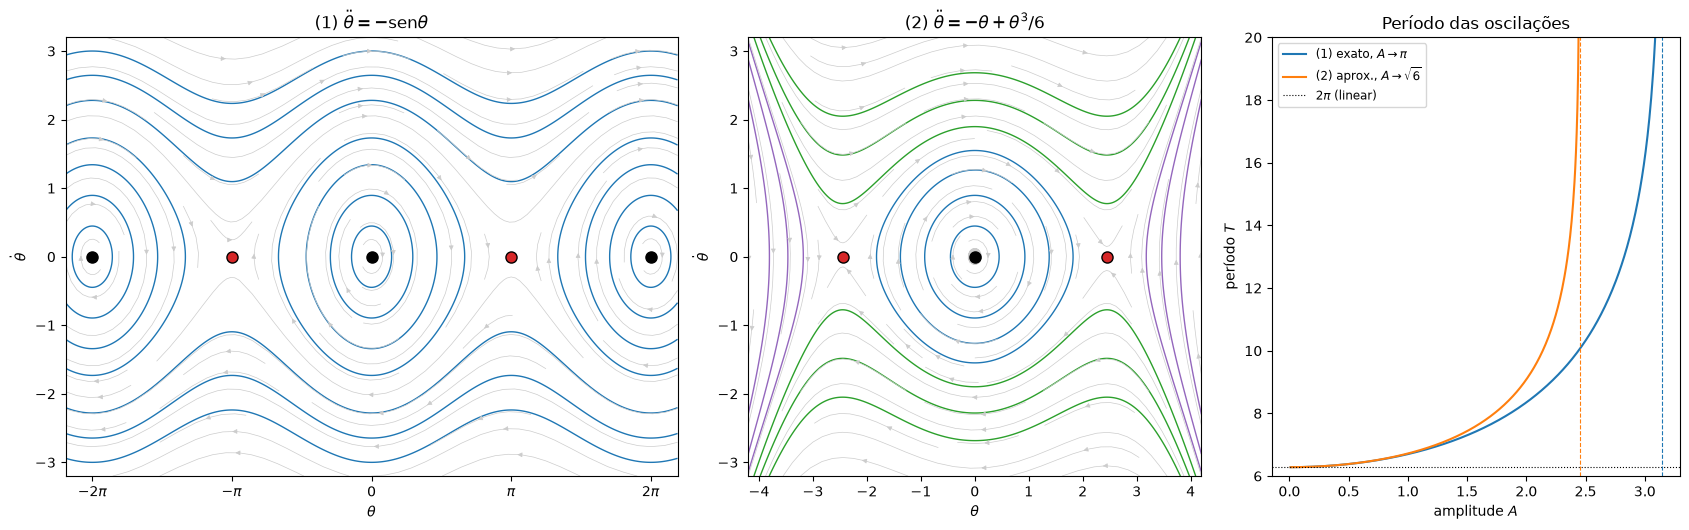
\includegraphics[width=0.5\linewidth]{2.png}
    \caption{Retratos de fase e comparação dos períodos.}
    \label{fig:2}
\end{figure}

\section{Mapa de grau 2}

\subsection{Expoente de Lyapunov nos regimes periódico e caótico}

\subsubsection{Séries temporais}

Os pontos fixos ocorrerão em $x^* = f(x^*) \iff b{x^*}^2+ x^* - 1 = 0 \Rightarrow x^* = \frac{-1 + \sqrt{1 + 4b}}{2b}$, para $x^* \in [-1,1]$. Assim, como $f'(x) = -2bx$, o mapa perde estabilidade quando $|f'(x)| < 1$, ou seja, $f'(x^*)= 1 - \sqrt{1 + 4b}$, mas, $f'(x) < 1$ $\forall b \in \langle 0, 2]$, então, a única fronteira que pode ser cruzada pelo mapa é em $-1$, que ocorre em $b = 3/4$. Como no intervalo $3/4 < b < 5/4$, $|4(1-b)|<1$, e o ciclo é estável. 

Considerando $x_0 = 0,1$, podemos esboçar as séries temporais para dois valores de $b$, $1,1$ e $1,9$, como na fig. \ref{fig:3ai}.

\begin{figure}[H]
    \centering
    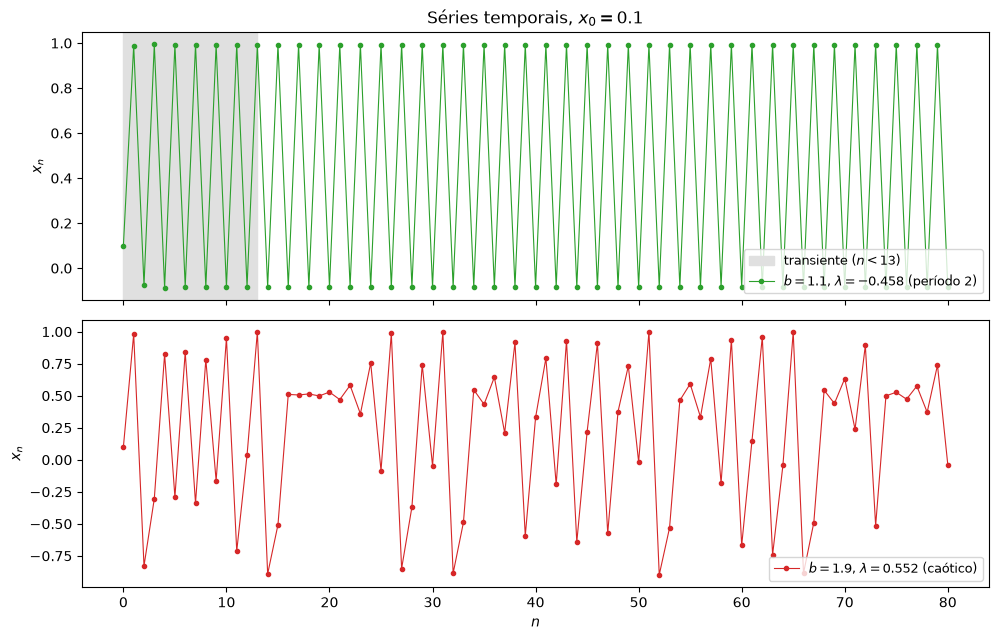
\includegraphics[width=0.5\linewidth]{3ai.png}
    \caption{Série temporal do mapa de grau 2.}
    \label{fig:3ai}
\end{figure}

\subsubsection{Expoente de Lyapunov e sensibilidade às condições iniciais}

Se considerarmos duas condições iniciais próximas, $x_0$ e $x_0'= x_0 + \delta_0$, para algum $|\delta_0| \ll 1$. Denominando $\delta_n := x_n'- x_n$ como a separação entre duas órbitas, podemos expandir um mapa $f(x)$ em torno de $x_n$ t.q. 

\[x'_{n+1}= f(x_n + \delta_n)= f(x_n) + f'(x_n)\delta_n + \mathcal{O}(\delta_n^2) \Rightarrow \delta_{n+1} \cong f'(x_n)\delta_n\]

Assim, se aplicarmos $\delta_1 \cong f'(x_0)\delta_0 $, e $\delta_2 \cong f(x_1)\delta_1 = f(x_1)f(x_0)\delta_0$, podemos, por indução, escrever 

\[\delta_{n+1} = \delta_0\prod_{k=0}^{n}f'(x_k)\]

Se escrevermos o produto na forma $|\delta_n| = |\delta_0|e^{\lambda n}$, 

\[\lambda = \lim_{n \to \infty}\frac{1}{n}\ln\bigg|\frac{\delta_n}{\delta_0}\bigg| = \lim_{n \to \infty}\frac{1}{n}\sum_{k=0}^{n-1}\ln|f'(x_k)|\]

que é o chamado expoente de Lyapunov. Com isso, conseguimos ter uma ideia de uma taxa média de separação por iteração passada, pensando computacionalmente. Para $\lambda <0$, órbitas vizinhas convergem para um mesmo ponto, mas, para $\lambda > 0$, as perturbações crescem exponencialmente, que é uma representação da sensibilidade às condições iniciais. Por exemplo, para o mapa de grau 2, podemos analisar esse distanciamento, como na fig. \ref{fig:3aii}. Nela, podemos ver que, para o sistema em regime caótico, as séries são praticamente indistinguíveis até $n \cong 35$, a partir do qual as trajetórias se distanciam significativamente. Isso pode, também, ser visualizado por meio do log-plot de $|\delta_n|$. 

O contrário também vale para o mapa com $b= 1,1$ e $\lambda = -0,46$, em que $|\delta_n|$ decai com $e^{\lambda n}$, de modo que as duas séries aparentem estarem sobrepostas durante todas as iterações. 

\begin{figure}[H]
    \centering
    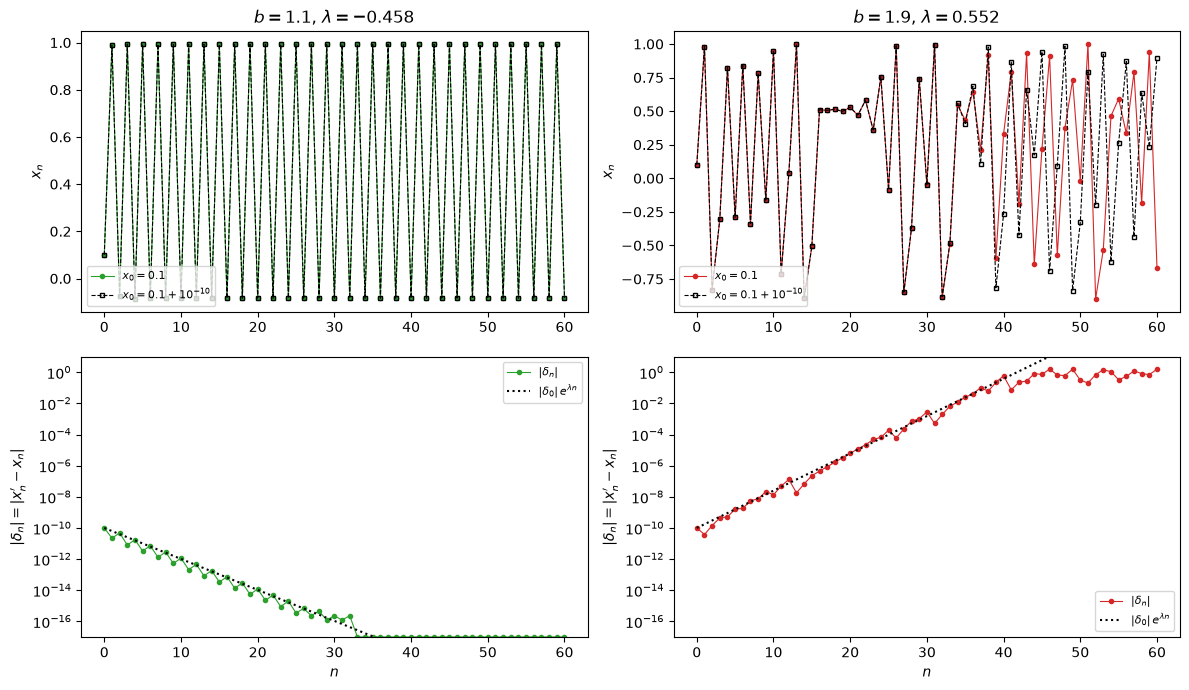
\includegraphics[width=0.5\linewidth]{3aii.png}
    \caption{Visualização da sensibilidade às condições iniciais.}
    \label{fig:3aii}
\end{figure}

\subsubsection{Diagramas de cobweb}

Podemos construir o diagrama de cobweb a partir de $x_{n+1} = 1 - bx_n^2$, e, a partir de $(x_0, 0)$, teremos, primeiro, um movimento vertical até a curva, mapeando $(x_n, f(x_n)) \to (x_n, x_{n+1})$, e um horizontal até a diagonal. Para ambos os casos discutidos previamente, temos os mapas da fig. 

\begin{figure}[H]
    \centering
    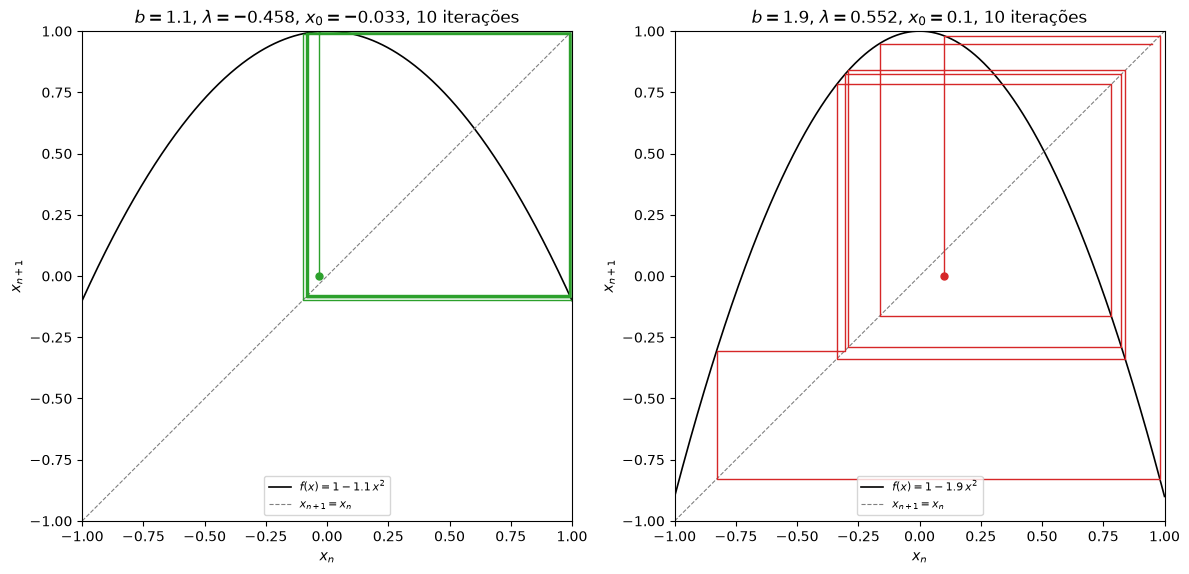
\includegraphics[width=0.5\linewidth]{3aiii.png}
    \caption{Diagrama de cobweb de ambos os casos, $b = 1,1$ e $b = 1,9$.}
    \label{fig:3aiii}
\end{figure}

\subsection{Rota para o caos por duplicação de período}

\subsubsection{Expoente de Lyapunov nas duplicações}

Se $\{x_j\}_{j=1}^p$ for um ciclo estável de período $p$, sobre ele, a soma que define o expoente de Lyapunov se repete a cada $p$ passos. Se definirmos 

\[\mu := \prod_{i=1}^p f'(x_i)\]

temos 

\[\lambda = \frac{1}{p}\ln|\mu|\]

O ciclo é estável quando $|\mu| < 1 \Rightarrow \lambda < 0$. No ponto da duplicação, $|\mu| = 1 \iff \lambda = 0$. Assim, em cada duplicação do período, o expoente de Lyapunov vai a zero. 

Podemos calcular numericamente os $b$'s em que isso acontece por meio do método de Newton aplicado às duplicações $f^{2^k}(x) - x$, e depois o método de Brent para solucionar $\mu_{2^k}(b) = -1$. Para as primeiras duas duplicações, teríamos $b_1 = 3/4$, como mencionado previamente, e $b_2 = 5/4$ de $\mu_2 = 4(1-b)=-1$.

Isso pode ser visualizado a partir de um diagrama de bifurcação, como na fig. \ref{fig:3bi_bif}.

\begin{figure}[H]
    \centering
    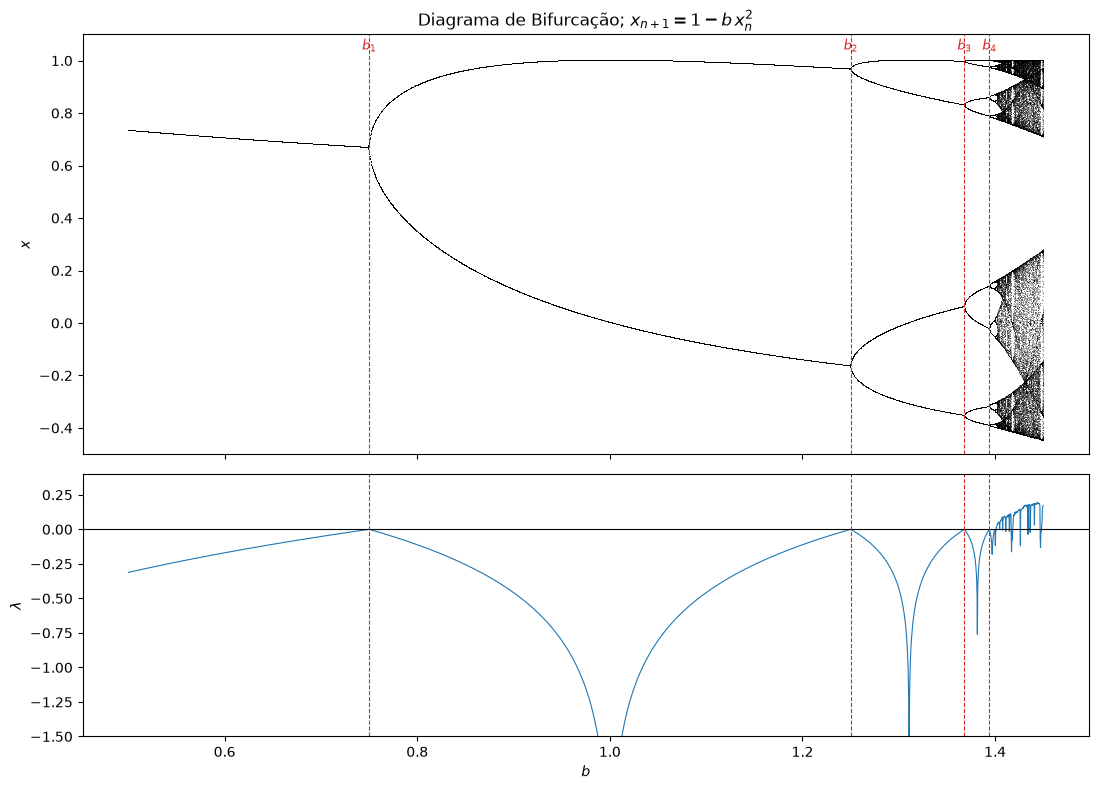
\includegraphics[width=0.5\linewidth]{3bi_bif.png}
    \caption{Diagrama de bifurcação do mapa quadrático.}
    \label{fig:3bi_bif}
\end{figure}

\subsection{Janelas periódicas imersas na região caótica}

\subsubsection{Janela de período 3}

Podemos encontrar as janelas periódicas considerando que um período pode ser definido como, após o transiente, o menor $p$ t.q. $|x_{n + p} - x_n| < 10^{-6}$, e colocando um máximo $p \leq 64$. Disso, se varrermos alguns valores de $b$, é possível encontrar a janela $1,75 < b < \sim1,77$ para o período 3. Disso, podemos dar um zoom na janela em questão, como na fig. \ref{fig:3ci}.

\begin{figure}[H]
    \centering
    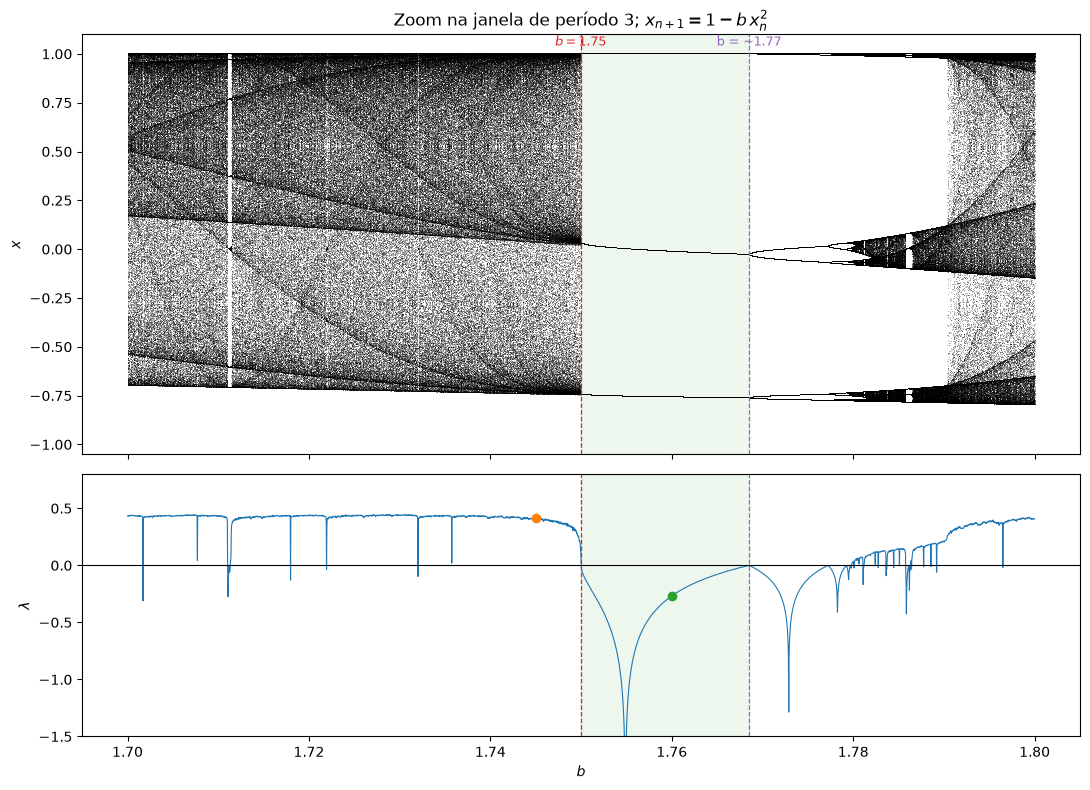
\includegraphics[width=0.5\linewidth]{3ci.png}
    \caption{Zoom na janela de período 3.}
    \label{fig:3ci}
\end{figure}

Podemos, também, visualizar as séries temporais correspondentes aos valores de $b$ identificados nos pontos da imagem na fig. \ref{fig:3ci_serie}.

\begin{figure}[H]
    \centering
    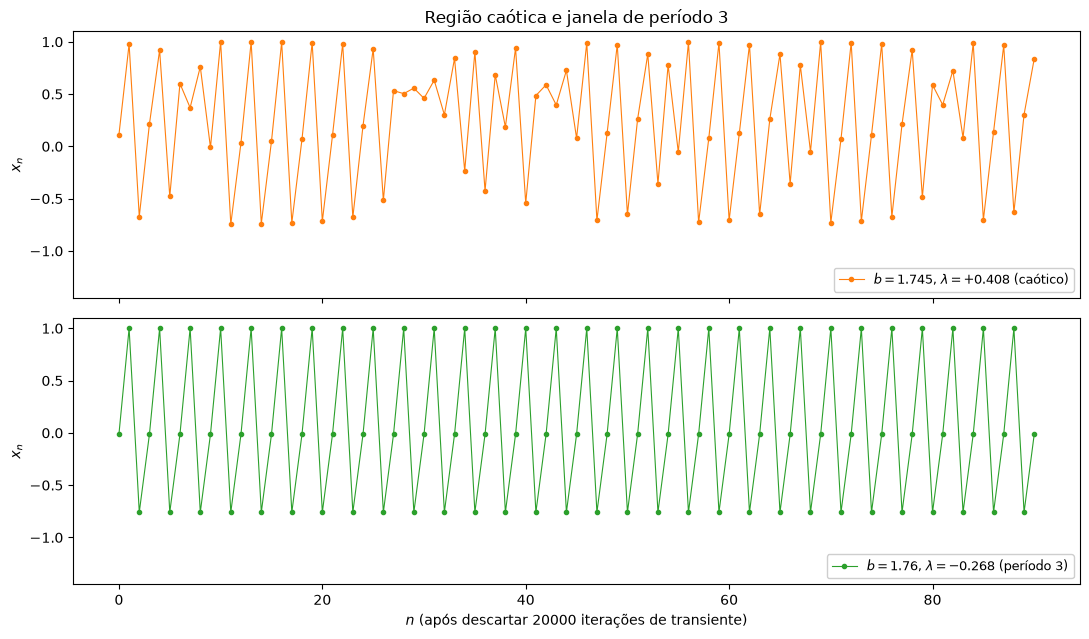
\includegraphics[width=0.5\linewidth]{3ci_serie.png}
    \caption{Séries temporais correspondentes a dois parâmetros de controle identificados na imagem.}
    \label{fig:3ci_serie}
\end{figure}

\subsubsection{Duplicação de período dentro da janela}

Do item anterior, o ciclo de período 3 deixa de ser estável em $b \sim1,77$\footnote{O valor com mais casas ($b = 1{,}76853$) foi utilizado nas contas, mas a ponta do intervalo foi mostrada dessa forma por brevidade.}, então, pelo mapa de bifurcação, conseguimos ver que haverá uma separação nesse ponto. Selecionando o intervalo $1{,}76853 \leq b \leq 1,790$, podemos utilizar o mesmo critério que em 3)c)i) para encontrar as duplicações e determinar a evolução ao caos. 

Para evitar que as duplicações fiquem comprimidas, são feitos zooms sucessivos, cada um de $b_k$ até um pouco depois de $b_{\infty}$, regime caótico. Como cada órbita de período $p$ percorre $p$ ramos, $x_n$ é marcado a cada $p$ iterações, e cada subplot mostra o ramo mais próximo de $x = 0$, por continuidade, com o eixo vertical sucessivamente ajustado. 

\begin{figure}[H]
    \centering
    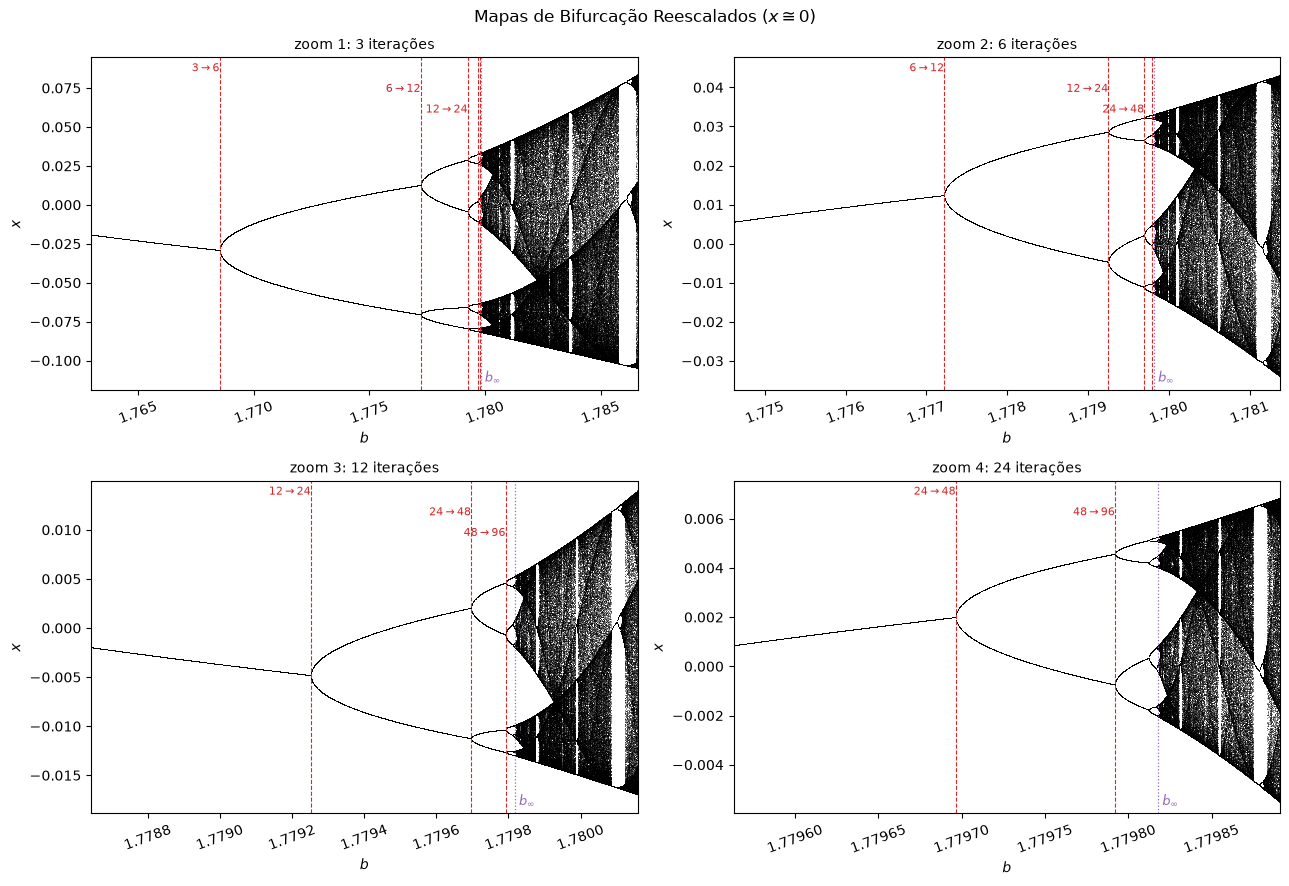
\includegraphics[width=0.5\linewidth]{3cii.png}
    \caption{Mapas de bifurcação sucessivamente ampliados.}
    \label{fig:3cii}
\end{figure}

Podemos observar a rota ao caos considerando o distanciamento de trajetórias próximas para alguns valores do parâmetro de controle no intervalo determinado, como na fig. \ref{fig:3cii_dist}. 

\begin{figure}[H]
    \centering
    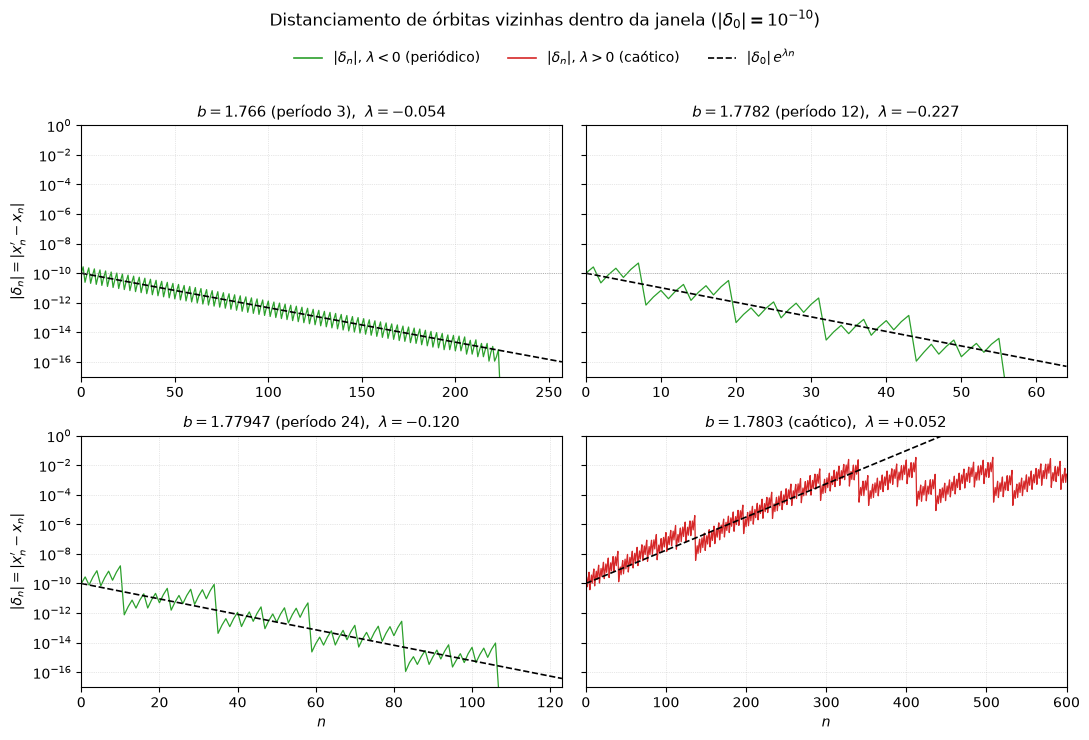
\includegraphics[width=0.5\linewidth]{3cii_distanciamento.png}
    \caption{Distanciamento de trajetórias próximas para 4 valores de $b$.}
    \label{fig:3cii_dist}
\end{figure}

\section{Duplicações de período e constante de Feigenbaum}

Os parâmetros $a_n$ são obtidos considerando que, para o ciclo de período $p = 2^{n-1}$, o método de Newton aplicado a $f^{p}(x) - x$ fornece o ciclo, e o
método de Brent resolve $\mu(a) = \prod_{i=1}^{p} f'(x_i) = -1$. 

A primeira duplicação é exata tanto no mapa fornecido quanto no mapa logístico visto que, para o mapa de grau 2, $f'(x^*) = 1 - \sqrt{1+4b} = -1 \iff b_1 = 3/4$, como visto previamente.

\begin{table}[H]
\centering
\caption{Duplicações de período para o mapa $f(x) = 1 - bx^2$.}
\begin{tabular}{c|ccc}
\hline
Períodos envolvidos na bifurcação & $b_n$ & $D_n = b_n - b_{n-1}$ & $\delta_n = D_{n-1}/D_n$ \\ \hline
$1 \Rightarrow 2$     & $3/4$ (exato) & ---          & ---      \\
$2 \Rightarrow 4$     & $5/4$ (exato) & $0{,}5$ (exato) & ---   \\
$4 \Rightarrow 8$     & $1{,}36809894$ & $0{,}11809894$ & $4{,}2337$ \\
$8 \Rightarrow 16$    & $1{,}39404616$ & $0{,}02594722$ & $4{,}5515$ \\
$16 \Rightarrow 32$   & $1{,}39963124$ & $0{,}00558508$ & $4{,}6458$ \\
$32 \Rightarrow 64$   & $1{,}40082874$ & $0{,}00119750$ & $4{,}6639$ \\
$64 \Rightarrow 128$  & $1{,}40108527$ & $0{,}00025653$ & $4{,}6681$ \\ \hline
\end{tabular}
\end{table}

No mapa em questão, $\delta_n$ tende à constante de Feigenbaum ($4{,}6692\ldots$).

\end{document}